\documentclass[journal,12pt,twocolumn]{IEEEtran}
%
\usepackage{setspace}
\usepackage{gensymb}
%\doublespacing
\singlespacing

%\usepackage{graphicx}
%\usepackage{amssymb}
%\usepackage{relsize}
\usepackage[cmex10]{amsmath}
%\usepackage{amsthm}
%\interdisplaylinepenalty=2500
%\savesymbol{iint}
%\usepackage{txfonts}
%\restoresymbol{TXF}{iint}
%\usepackage{wasysym}
\usepackage{amsthm}
%\usepackage{iithtlc}
\usepackage{mathrsfs}
\usepackage{txfonts}
\usepackage{stfloats}
\usepackage{bm}
\usepackage{cite}
\usepackage{cases}
\usepackage{subfig}
%\usepackage{xtab}
\usepackage{longtable}
\usepackage{multirow}
%\usepackage{algorithm}
%\usepackage{algpseudocode}
\usepackage{enumitem}
\usepackage{mathtools}
\usepackage{tikz}
\usepackage{circuitikz}
\usepackage{verbatim}
\usepackage{tfrupee}
\usepackage[breaklinks=true]{hyperref}
%\usepackage{stmaryrd}
\usepackage{tkz-euclide} % loads  TikZ and tkz-base
\usetkzobj{all}
\usetikzlibrary{decorations.markings}
\usetikzlibrary{shapes.geometric}
\newif\iflabrev
\usepackage{listings}
    \usepackage{color}                                            %%
    \usepackage{array}                                            %%
    \usepackage{longtable}                                        %%
    \usepackage{calc}                                             %%
    \usepackage{multirow}                                         %%
    \usepackage{hhline}                                           %%
    \usepackage{ifthen}                                           %%
  %optionally (for landscape tables embedded in another document): %%
    \usepackage{lscape}     
\usepackage{multicol}
\usepackage{chngcntr}
\usetikzlibrary{shapes,arrows}
%\usepackage{enumerate}

%\usepackage{wasysym}
%\newcounter{MYtempeqncnt}
\DeclareMathOperator*{\Res}{Res}
%\renewcommand{\baselinestretch}{2}
\renewcommand\thesection{\arabic{section}}
\renewcommand\thesubsection{\thesection.\arabic{subsection}}
\renewcommand\thesubsubsection{\thesubsection.\arabic{subsubsection}}

\renewcommand\thesectiondis{\arabic{section}}
\renewcommand\thesubsectiondis{\thesectiondis.\arabic{subsection}}
\renewcommand\thesubsubsectiondis{\thesubsectiondis.\arabic{subsubsection}}

% correct bad hyphenation here
\hyphenation{op-tical net-works semi-conduc-tor}
\def\inputGnumericTable{}                                 %%

\lstset{
%language=C,
frame=single, 
breaklines=true,
columns=fullflexible
}
%\lstset{
%language=tex,
%frame=single, 
%breaklines=true
%}

\begin{document}
%


\newtheorem{theorem}{Theorem}[section]
\newtheorem{problem}{Problem}
\newtheorem{proposition}{Proposition}[section]
\newtheorem{lemma}{Lemma}[section]
\newtheorem{corollary}[theorem]{Corollary}
\newtheorem{example}{Example}[section]
\newtheorem{definition}[problem]{Definition}
%\newtheorem{thm}{Theorem}[section] 
%\newtheorem{defn}[thm]{Definition}
%\newtheorem{algorithm}{Algorithm}[section]
%\newtheorem{cor}{Corollary}
\newcommand{\BEQA}{\begin{eqnarray}}
\newcommand{\EEQA}{\end{eqnarray}}
\newcommand{\define}{\stackrel{\triangle}{=}}
\bibliographystyle{IEEEtran}
%\bibliographystyle{ieeetr}
\providecommand{\mbf}{\mathbf}
\providecommand{\pr}[1]{\ensuremath{\Pr\left(#1\right)}}
\providecommand{\qfunc}[1]{\ensuremath{Q\left(#1\right)}}
\providecommand{\sbrak}[1]{\ensuremath{{}\left[#1\right]}}
\providecommand{\lsbrak}[1]{\ensuremath{{}\left[#1\right.}}
\providecommand{\rsbrak}[1]{\ensuremath{{}\left.#1\right]}}
\providecommand{\brak}[1]{\ensuremath{\left(#1\right)}}
\providecommand{\lbrak}[1]{\ensuremath{\left(#1\right.}}
\providecommand{\rbrak}[1]{\ensuremath{\left.#1\right)}}
\providecommand{\cbrak}[1]{\ensuremath{\left\{#1\right\}}}
\providecommand{\lcbrak}[1]{\ensuremath{\left\{#1\right.}}
\providecommand{\rcbrak}[1]{\ensuremath{\left.#1\right\}}}
\theoremstyle{remark}
\newtheorem{rem}{Remark}
\newcommand{\sgn}{\mathop{\mathrm{sgn}}}
\providecommand{\abs}[1]{\left\vert#1\right\vert}
\providecommand{\res}[1]{\Res\displaylimits_{#1}} 
\providecommand{\norm}[1]{\left\lVert#1\right\rVert}
%\providecommand{\norm}[1]{\lVert#1\rVert}
\providecommand{\mtx}[1]{\mathbf{#1}}
\providecommand{\mean}[1]{E\left[ #1 \right]}
\providecommand{\fourier}{\overset{\mathcal{F}}{ \rightleftharpoons}}
%\providecommand{\hilbert}{\overset{\mathcal{H}}{ \rightleftharpoons}}
\providecommand{\system}{\overset{\mathcal{H}}{ \longleftrightarrow}}
	%\newcommand{\solution}[2]{\textbf{Solution:}{#1}}
\newcommand{\solution}{\noindent \textbf{Solution: }}
\newcommand{\cosec}{\,\text{cosec}\,}
\providecommand{\dec}[2]{\ensuremath{\overset{#1}{\underset{#2}{\gtrless}}}}
\newcommand{\myvec}[1]{\ensuremath{\begin{pmatrix}#1\end{pmatrix}}}
\newcommand{\mydet}[1]{\ensuremath{\begin{vmatrix}#1\end{vmatrix}}}
%\numberwithin{equation}{section}
\numberwithin{equation}{subsection}
%\numberwithin{problem}{section}
%\numberwithin{definition}{section}
\makeatletter
\@addtoreset{figure}{problem}
\makeatother
\let\StandardTheFigure\thefigure
\let\vec\mathbf
%\renewcommand{\thefigure}{\theproblem.\arabic{figure}}
\renewcommand{\thefigure}{\theproblem}
%\setlist[enumerate,1]{before=\renewcommand\theequation{\theenumi.\arabic{equation}}
%\counterwithin{equation}{enumi}
%\renewcommand{\theequation}{\arabic{subsection}.\arabic{equation}}
\def\putbox#1#2#3{\makebox[0in][l]{\makebox[#1][l]{}\raisebox{\baselineskip}[0in][0in]{\raisebox{#2}[0in][0in]{#3}}}}
     \def\rightbox#1{\makebox[0in][r]{#1}}
     \def\centbox#1{\makebox[0in]{#1}}
     \def\topbox#1{\raisebox{-\baselineskip}[0in][0in]{#1}}
     \def\midbox#1{\raisebox{-0.5\baselineskip}[0in][0in]{#1}}
\vspace{3cm}
\title{
%	\logo{
Control Systems
%	}
}
\author{ G V V Sharma$^{*}$% <-this % stops a space
	\thanks{*The author is with the Department
		of Electrical Engineering, Indian Institute of Technology, Hyderabad
		502285 India e-mail:  gadepall@iith.ac.in. All content in this manual is released under GNU GPL.  Free and open source.}
	
}	
%\title{
%	\logo{Matrix Analysis through Octave}{\begin{center}\includegraphics[scale=.24]{tlc}\end{center}}{}{HAMDSP}
%}
% paper title
% can use linebreaks \\ within to get better formatting as desired
%\title{Matrix Analysis through Octave}
%
%
% author names and IEEE memberships
% note positions of commas and nonbreaking spaces ( ~ ) LaTeX will not break
% a structure at a ~ so this keeps an author's name from being broken across
% two lines.
% use \thanks{} to gain access to the first footnote area
% a separate \thanks must be used for each paragraph as LaTeX2e's \thanks
% was not built to handle multiple paragraphs
%
%\author{<-this % stops a space
%\thanks{}}
%}
% note the % following the last \IEEEmembership and also \thanks - 
% these prevent an unwanted space from occurring between the last author name
% and the end of the author line. i.e., if you had this:
% 
% \author{....lastname \thanks{...} \thanks{...} }
%                     ^------------^------------^----Do not want these spaces!
%
% a space would be appended to the last name and could cause every name on that
% line to be shifted left slightly. This is one of those "LaTeX things". For
% instance, "\textbf{A} \textbf{B}" will typeset as "A B" not "AB". To get
% "AB" then you have to do: "\textbf{A}\textbf{B}"
% \thanks is no different in this regard, so shield the last } of each \thanks
% that ends a line with a % and do not let a space in before the next \thanks.
% Spaces after \IEEEmembership other than the last one are OK (and needed) as
% you are supposed to have spaces between the names. For what it is worth,
% this is a minor point as most people would not even notice if the said evil
% space somehow managed to creep in.
% The paper headers
%\markboth{Journal of \LaTeX\ Class Files,~Vol.~6, No.~1, January~2007}%
%{Shell \MakeLowercase{\textit{et al.}}: Bare Demo of IEEEtran.cls for Journals}
% The only time the second header will appear is for the odd numbered pages
% after the title page when using the twoside option.
% 
% *** Note that you probably will NOT want to include the author's ***
% *** name in the headers of peer review papers.                   ***
% You can use \ifCLASSOPTIONpeerreview for conditional compilation here if
% you desire.
% If you want to put a publisher's ID mark on the page you can do it like
% this:
%\IEEEpubid{0000--0000/00\$00.00~\copyright~2007 IEEE}
% Remember, if you use this you must call \IEEEpubidadjcol in the second
% column for its text to clear the IEEEpubid mark.
% make the title area
\maketitle
\newpage
\tableofcontents
\bigskip
\renewcommand{\thefigure}{\theenumi}
\renewcommand{\thetable}{\theenumi}
%\renewcommand{\theequation}{\theenumi}
%\begin{abstract}
%%\boldmath
%In this letter, an algorithm for evaluating the exact analytical bit error rate  (BER)  for the piecewise linear (PL) combiner for  multiple relays is presented. Previous results were available only for upto three relays. The algorithm is unique in the sense that  the actual mathematical expressions, that are prohibitively large, need not be explicitly obtained. The diversity gain due to multiple relays is shown through plots of the analytical BER, well supported by simulations. 
%
%\end{abstract}
% IEEEtran.cls defaults to using nonbold math in the Abstract.
% This preserves the distinction between vectors and scalars. However,
% if the journal you are submitting to favors bold math in the abstract,
% then you can use LaTeX's standard command \boldmath at the very start
% of the abstract to achieve this. Many IEEE journals frown on math
% in the abstract anyway.
% Note that keywords are not normally used for peerreview papers.
%\begin{IEEEkeywords}
%Cooperative diversity, decode and forward, piecewise linear
%\end{IEEEkeywords}
% For peer review papers, you can put extra information on the cover
% page as needed:
% \ifCLASSOPTIONpeerreview
% \begin{center} \bfseries EDICS Category: 3-BBND \end{center}
% \fi
%
% For peerreview papers, this IEEEtran command inserts a page break and
% creates the second title. It will be ignored for other modes.
%\IEEEpeerreviewmaketitle
\begin{abstract}
This manual is an introduction to control systems based on GATE problems.Links to sample Python codes are available in the text.  
\end{abstract}
Download python codes using 
\begin{lstlisting}
svn co https://github.com/gadepall/school/trunk/control/codes
\end{lstlisting}
%\section{Mason's Gain Formula}
%\section{Bode Plot}
%\subsection{Introduction}
%\subsection{Example}
%\section{Second order System}
%\subsection{Damping}
%\subsection{Example}
%\section{Routh Hurwitz Criterion}
%\subsection{Routh Array}
%\subsection{Marginal Stability}
%\subsection{Stability}
%\input{./chapters/EE18BTECH11021.tex}
%\section{State-Space Model}
%\input{./chapters/ee18btech11004.tex}
%\subsection{Second Order System}
%\section{Nyquist Plot}
%\section{Phase Margin}
%\section{Gain Margin}
%\section{Compensators}
%\subsection{Phase Lead}
%\input{./chapters/EE18BTECH11021_2.tex}
%\section{Oscillator}
\section{Compensators}
\begin{enumerate}[label=\thesection.\arabic*.,ref=\thesection.\theenumi]
\numberwithin{equation}{enumi}

\item For a unity feedback system shown in \ref{fig:ee18btech11044_1}, $\frac{10}{s(s+1)}$. Design a lead compensator such that the phase margin of the system is 45$^{\circ}$ and appropriate steady state error is less than or equal to $\frac{1}{15}$ units of the final output value. Further the gain crossover frequency of the system must be less than 7.5rad/sec. \\


\item For the control system shown in \ref{fig:ee18btech11044_1} write the steady state output for step input. \\
\solution
\begin{align}
\lim_{t\to\infty} y(t)  = \lim_{s\to0} sY(s) \\
\lim_{s\to0} sY(s) = \lim_{s\to0}  \frac{s R(s) G(s)}{1+G(s)} \\
\lim_{s\to0} sY(s) = \lim_{s\to0} \frac{G(s)}{1 + G(s)}
\end{align}
\begin{figure}[!ht]
	\begin{center}
		\resizebox{\columnwidth}{!}{\tikzstyle{block} = [draw, fill=white, rectangle, 
    minimum height=1cm, minimum width=1cm]
\tikzstyle{sum} = [draw, fill=white, circle, node distance=1cm]
\tikzstyle{input} = [coordinate]
\tikzstyle{output} = [coordinate]
\tikzstyle{pinstyle} = [pin edge={to-,thin,black}]


% The block diagram code is probably more verbose than necessary
\begin{tikzpicture}[auto, node distance=2cm,>=latex']
    % We start by placing the blocks
    \node [input, name=input] {X(s)};
    \node [sum, right of=input] (sum) {};
    
    \node [block, right of=sum] (system) {$G(s)$ };
   
    % We draw an edge between the controller and system block to 
    % calculate the coordinate u. We need it to place the measurement block. 
    
    \node [output, right of=system] (output) {};
    \node [block, below of=system] (measurements) {1};

    % Once the nodes are placed, connecting them is easy. 
    \draw [draw,->] (input) -- node {$R(s)$} (sum);
    \draw [->] (sum) -- node {} (system);
    \draw [->] (system) -- node [name=y] {$Y(s)$}(output);
    \draw [->] (y) |- (measurements);
    \draw [->] (measurements) -| node[pos=0.99] {$-$} 
        node [near end] {} (sum);
\end{tikzpicture}
}
	\end{center}
\caption{}
\label{fig:ee18btech11044_1}
\end{figure}

\item What do you mean by steady state error and write the expression for steady state error for control system shown in \ref{fig:ee18btech11044_1} considering step input. \\
\solution 
Steady-state error is the difference between the input and the output for a prescribed test input as time tends to infinity.
\begin{align}
    e_{ss} = \lim_{s\to0} \frac{1}{1 +G(s)}
\end{align}


\item Write the general expression for the transfer function of a phase lead compensator. \\
\solution 
\begin{align}
    G_c(s) =  K_{comp}    \frac{(1+\alpha T s)}{(1+ T s)} 
\end{align}
\ref{fig:ee18btech11044_2} shows the compensated control system.
\begin{figure}[!ht]
	\begin{center}
		\resizebox{\columnwidth}{!}{\tikzstyle{block} = [draw, fill=white, rectangle, 
    minimum height=1cm, minimum width=1cm]
\tikzstyle{sum} = [draw, fill=white, circle, node distance=1cm]
\tikzstyle{input} = [coordinate]
\tikzstyle{output} = [coordinate]
\tikzstyle{pinstyle} = [pin edge={to-,thin,black}]


% The block diagram code is probably more verbose than necessary
\begin{tikzpicture}[auto, node distance=2cm,>=latex']
    % We start by placing the blocks
    \node [input, name=input] {X(s)};
    \node [sum, right of=input] (sum) {};
    
    \node [block, right of=sum] (system) {$G(s)$ };
   
    % We draw an edge between the controller and system block to 
    % calculate the coordinate u. We need it to place the measurement block. 
    
    \node [output, right of=system] (output) {};
    \node [block, below of=system] (measurements) {1};

    % Once the nodes are placed, connecting them is easy. 
    \draw [draw,->] (input) -- node {$R(s)$} (sum);
    \draw [->] (sum) -- node {} (system);
    \draw [->] (system) -- node [name=y] {$Y(s)$}(output);
    \draw [->] (y) |- (measurements);
    \draw [->] (measurements) -| node[pos=0.99] {$-$} 
        node [near end] {} (sum);
\end{tikzpicture}
}
	\end{center}
\caption{}
\label{fig:ee18btech11044_2}
\end{figure}


\item Calculate the steady state output value and steady state error for the control system shown in \ref{fig:ee18btech11044_1}, where G(s) = $\frac{10}{s(s+1)}$. Consider the input to be unit step. \\
\solution \\
\textbf{Steady state value:}
\begin{align}
\lim_{t\to\infty} y(t) = \lim_{s\to0} \frac{10}{10+s(s+1)} \\
\lim_{t\to\infty} y(t) = 1
\end{align}
\textbf{Steady state error:}
\begin{align}
e_{ss} = \lim_{s\to0} \frac{s(s+1)}{10 + s(s+1)} \\
e_{ss} = 0
\end{align}

\item Choose a value of $K_{comp}$ which satisfies the steady state error condition. \\
\solution As the steady state error for unit step response is always zero, any value of $K_{comp}$ satisfies the steady state error condition in compensated system. For simplicity let us choose $K_{comp}$ = 1.

\item Calculate phase margin and gain cross over frequency of open-loop transfer function G(S). \\
\solution \\
\textbf{Gain cross over frequency}:
\begin{align}
    G(j\omega) = \frac{10}{j\omega (j\omega + 1)} \\
    |G(j\omega)| = \frac{10}{\sqrt{\omega^4 +\omega^2}} \\
    \frac{10}{\sqrt{\omega^4 +\omega^2}} = 1 \\
    \omega_{gc} = 3.084
\end{align}
\textbf{Phase Margin}:
\begin{align}
    \phi =  -90^{\circ} - tan^{-1}(\omega) \\ 
    pm = 180^{\circ} -90^{\circ} - tan^{-1}(\omega_{gc}) \\ 
    pm = 17.966^{\circ} \\ 
\end{align}
\item Write the expression for maximum phase of a lead compensator and the frequency where it occurs \\
\solution 
\begin{align}
    \phi_{max} = sin^{-1}(\frac{\alpha - 1}{\alpha + 1}) \label{eq:ee18btech11044_1} \\
    \omega_m = \frac{1}{T \alpha} \label{eq:ee18btech11044_2}
\end{align}

\item Calculate the value of $\phi_{max}$ required to meet desired phase margin. \\
\solution 
\begin{align}
    \phi_{max} = 45^{\circ} - pm + 15^{\circ} \\ 
    \phi_{max} = 45^{\circ} - 17.966^{\circ} + 15^{\circ} \\
    \phi_{max} = 42.034^{\circ}
\end{align}
Here the extra $15^o$ has been added to compensate for the shift in $\omega_{gc}$.  
\item Using \eqref{eq:ee18btech11044_1} calculate the value of $\alpha$ \\
\solution 
\begin{align}
    sin(42.034^{\circ}) = \frac{\alpha - 1}{\alpha + 1} \\
    0.669 = \frac{\alpha - 1}{\alpha + 1} \\ 
    0.331 \alpha = 1.669 \\
    \alpha = 5.04
\end{align}
\item Choose appropriate value for $\omega_m$. \\
\solution 
\begin{itemize}
    \item For maximum increase in phase margin we have to ensure that $\phi_{max}$ occurs at frequency close to $\omega_{gc}$ of G(s).
    \begin{align}
        \omega_m = 3.084 rad/sec
    \end{align}
    \item We know that $\omega_{gc}$ gets shifted slightly when we cascade a compensator to original transfer function, to compensate for the shift we have already added an extra $15^{\circ}$ to $\phi_{max}$.
\end{itemize}

\item Using \eqref{eq:ee18btech11044_2} calculate the value of T. \\
\solution
\begin{align}
    T = \frac{1}{ \omega_m \alpha} \\
    T = \frac{1}{15.54} \\
    T = 0.064
\end{align}

\item Write the final expression of the Lead compensator designed. \\
\solution
\begin{align}
    G_c(s) =   \frac{(1+ 0.322 s)}{(1+ 0.064 s)} 
\end{align}
\begin{itemize}
    \item Zero at s = -3.084
    \item Pole at s = -15.54
\end{itemize}
\item Verify using a python plot. \\
\solution
\begin{lstlisting}
codes/ee18btech11044_2.py
\end{lstlisting}

\begin{figure}[!ht]
\centering
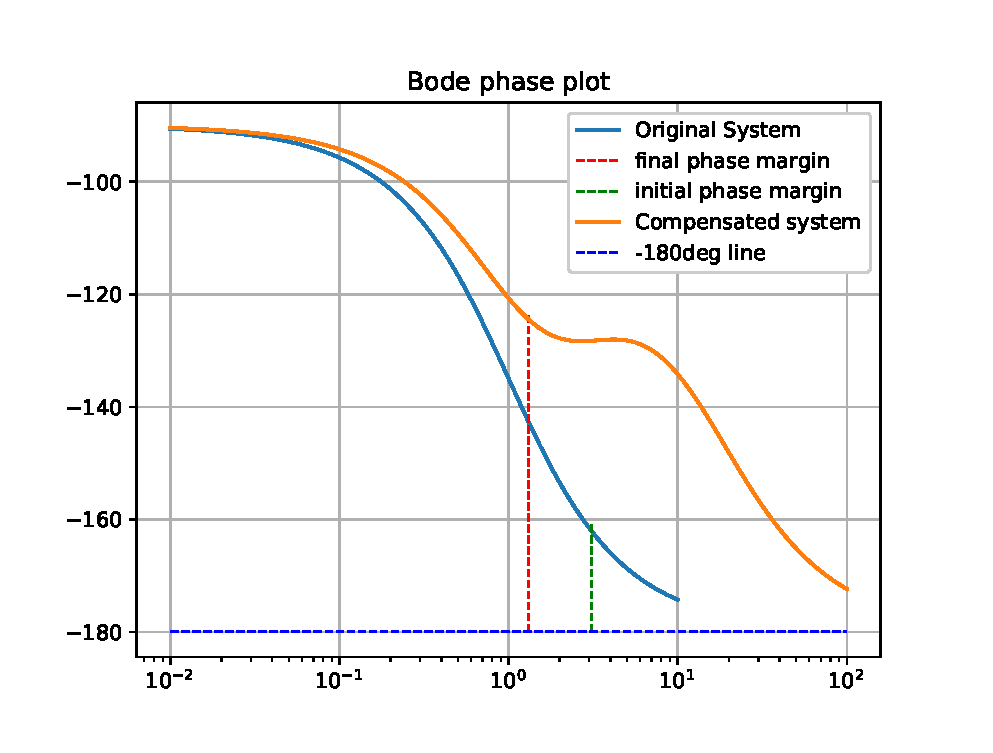
\includegraphics[width=\columnwidth]{figs/ee18btech11044_2_1.eps}
\caption{}
\end{figure}
\end{enumerate}


\end{document}
